\documentclass[10pt, conference, compsocconf]{IEEEtran}
\usepackage{csquotes}
\usepackage{epigraph}
\usepackage{graphicx}
\graphicspath{ {graphics/} }
\renewcommand\IEEEkeywordsname{Keywords}
\renewcommand{\figurename}{Figure}

\begin{document}

\title{Adaptive Indexing: Cracking Facts and Merging Knowledge}
\author{Pavlo Shevchenko \\ Otto-von-Guericke-University, Magdeburg \\ pavlo.shevchenko@st.ovgu.de}

\maketitle

\epigraph{Therefore, even as an index to a book \\
So to his mind was young Leander's look}{\textit{Christopher Marlowe\\Hero and Leander, 1593}}

\begin{abstract}
Database indexes have been used in database systems for a long time. They provide necessary functionality to quickly access relevant tuples of data. In this paper, we review an advanced indexing concept, known as \emph{adaptive indexing}, which promotes the idea that index creation is a part of query processing. We revisit basic approaches for adaptive indexing: \emph{database cracking} and \emph{adaptive indexing}. We discuss issues of these methods and review proposed modifications, known as \emph{hybrid approaches} that combine strengh of both approaches. As a result, we provide a complete overview of the core concepts of adaptive indexing, lay down some background for further research and outline issues that remain unsolved.\\
\end{abstract}

\begin{IEEEkeywords}
Database indexing, adaptive indexing, database cracking, adaptive merging, hybrid approaches.
\end{IEEEkeywords}

\section{Introduction}
The concept of indexes was widely used in the library science throughout the history of mankind and remains the main tool to help the reader find information quickly. Indexes easily made their way into database technologies. The introduction of such intuitive concept helped to improve the speed of data retrieval. In the early stages of database technology, data and indexes were stored on disk in a form of B-Trees. These datastructures, optimized for these purposes, enable efficient usage of disk pages and management of data stored in disk.

However, over the years, as in-memory databases (IMDB) found their way to the market, the need for more lightweight index structures has become evident. At first, a precalculated index in a form of a sorted column with pointers to the original records in the table has become a concept that helped to decrease the query response time. However, continuously growing amount of data, more sophisticated queries and unpredictable behavior of a user have turned advantages of indexes into disadvantages\cite{partial2}. Storing large columns in a main memory has become a problem, the need to store indexes to numerous columns has even increased that problem. As it is hard to predict which column is especially interesting for the user, new indexes have to be calculated online as queries referring to new columns arrive.

All these issues motivated the development of advanced indexing techniques such as \emph{partial} \cite{partial1} and \emph{soft} \cite{soft_indexes} indexes. We discuss both these concepts in detail in Section~\ref{sec:background}. Creators of the latter realised that an index cannot remain static after being created, it requires to be continuously tuned as some parameters of the database system are changing. Such parameters include workload, size and distribution of data, schema and infrastructure changes \cite{soft_indexes}. Currently, indexes are tuned by DBA with help of some management tools that provide this information to system administrators. However, it is desired that database tuning is performed by DBMS alone (like it is already done for storage layout, access optimization, etc.). Statistical data mentioned before is collected during query processing. Therefore, as new queries arrive, DBMS can adapt existing indexes or create new ones on-the-fly, depending on how these parameters have changed \cite{soft_indexes}.

This concept known as adaptive indexing will be presented in this short paper. We revisit some fundamental approaches (e.g. \emph{database cracking} \cite{cracking} and \emph{adaptive merging} \cite{merging}) in Sections~\ref{sec:cracking} and~\ref{sec:merging} respectively. Further approaches that try to combine the advantages of both methods will be introduced in Section~\ref{sec:hybrid}. We evaluate the presented approaches in Section~\ref{sec:eval}. We conclude this paper by reviewing related work in Section~\ref{sec:rel} and proposing directions for further research in Section~\ref{sec:conc}.

Our goal is to provide a complete overview of adaptive indexing techniques to help everyone interested in them understand the core concepts of the approaches. Furthermore, we aim to draw attention to these techniques and motivate further studies in the area of adaptive indexing.

\section{Background}
\label{sec:background}
As mentioned before, two indexing methods: partial indexes \cite{partial1} and soft indexes \cite{soft_indexes} were developed to tackle some problems caused by traditional indexes. In this section, both of these approaches and their influence on adaptive indexing will be presented.
\subsection{Partial Indexes}
\label{subsec:partial}
As its name suggests, a partial index, also known as a filtered index, is an index which contains only part of the indexed column that satisfies some condition. Such condition is usually expressed in the form of an interval known as \emph{inclusion interval}. Depending on selectivity of a condition, the amount of rows in the indexed column can be decreased. This allows to reduce the amount of memory needed to store the index. The creation of such index may be specified as follows:
\begin{displayquote}
\texttt{CREATE \hspace{0.2 cm} INDEX \hspace{0.2 cm} ON \hspace{0.2 cm} relation(column) name \\ WHERE \hspace{0.2 cm} condition}
\end{displayquote}

In Figure 1, we present an example of a partial index with a condition $'D' \leq A \leq 'O'$. Next to it, we give an example of a full index to a given table.

Clearly, selecting the right condition is a key element for the creation of a partial index. This condition can be found in several ways:\\
\begin{itemize}

\item{User Input \cite{partial1}:}\\ User can specify the insertion interval while possessing some additional knowledge about the data. However, one of the major principles of modern DBMS is removing any low-level data management aspects from the user of the system. As a result, DBMS should be able to derive such conditions itself.\\

\item{Index Creation as Side-Effect of Query Processing \cite{partial1}:}\\ Even though the user has been removed from tuning process, she can still indirectly participate in finding a suitable condition. The fact that user queries some relation (column) while applying some selection condition, leads to an assumption that this part of data is of some interest for the user and may be queried again in the future. So, taking query condition from the user as a qualification for partial index is not a bad idea after all. Continuous refinement of a condition and ad-hoc indexing may provide an optimal partial index for given relation. This concept, known as \emph{online index creation} was later used in database cracking \cite{cracking}.\\

\item{Statistical Approach \cite{partial2}:} \\Since index creation in a way described above may increase query processing time, statistical information, like the percentage of queries that access each column or distribution of values in each column, may be used to perform index creation after data loading and before queries are processed. In contrast to previous concept, this approach is known as \emph{offline index creation}, as the index is not created during query processing, but before.
\end{itemize}

\begin{figure}[h]
\centering
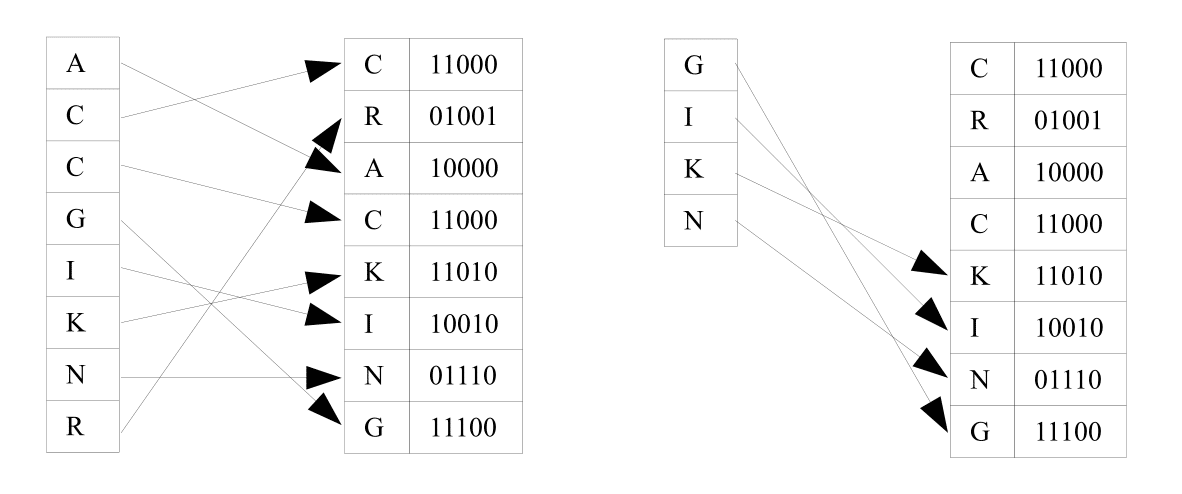
\includegraphics[width=\columnwidth]{partial.png}
\caption{Full Index (left) and Partial Index (right)}
\end{figure}

\subsection{Soft Indexes}
\label{subsec:soft}
In contrast to \emph{hard indexes} that are created by database assistant and stored as long as he wants to, soft indexes proposed in \cite{soft_indexes} are created, modified and dropped by DBMS depending on the current configuration of the system. Index management is carried out in three major steps:
\begin{itemize}
\item{Observation}
\item{Prediction}
\item{Reaction}
\end{itemize}

At first, statistical information about current state of the system (workload, data, schema, infrastructure) is collected in the Observation phase. In the Prediction phase, a list of index candidates sorted by some criteria is analyzed and top \textit{k} candidates are chosen for later materilization. During the Reaction phase, depending on results of Prediction phase, some indexes will be created or deleted \cite{soft_indexes}.\\

\textbf{Value}. Combination of advantages of soft and partial indexes resulted in further approaches known as adaptive indexing. This concept promotes the idea of completely automative tuning process of a database system. Adaptive indexing achieves it by continuously reorganising physical design of a database system during incremental and partial online indexing \cite{defin}. On-the-fly index creation based on the query workload and storing only subsets of rows in an index motivated the first method for adaptive indexing, called \emph{database cracking} \cite{cracking}, which we present in the next section.

\section{Database Cracking}
\label{sec:cracking}
After presenting the necessary background about partial and soft indexes, we revisit one of the main approaches of adaptive indexing, database cracking. In Subsection~\ref{subsec:crack_idea} we discuss main idea behind database cracking, in Subsection~\ref{subsec:st_crack} we revisit the standard cracking algorithm. In Figure 2, we give an example of how the described algorithm can be used. To conclude this section, we analyze database cracking and compare it to full index and full scan.

\subsection{Motivation and Basic Idea}
\label{subsec:crack_idea}
\textbf{Motivation}. Database cracking is pursuing the goal to provide fast access to the data and the self-organized behavior of database system. It is based on idea that index maintenance is a byproduct of query processing, not updates \cite{cracking}. In contrast to soft indexes, discussed earlier, database cracking achieves its goal not by tuning system's configuration and choosing the best fitting indexes based on numerous parameters, but by using continuous physical reorganization (cracking the database into manageable pieces).

\subsection{Standard Cracking}
\label{subsec:st_crack}
\textbf{Main Idea}: \textit{incrementally perform quicksort on a copy of a column using crack-in-three when range query fully falls in the same partition and crack-in-two otherwise.}\\

\textbf{Crack-In-Two}: \textit{partition the index column into two pieces using range as a split line.}\\

\textbf{Crack-In-Three}: \textit{partition the index column into three pieces using ends of a range as two split lines.}\\

\textbf{Steps of Standard Cracking} (given a column-oriented database with column \textit{A}; range query \textit{q} in a form of either \textit{$c \leq R.A$} or \textit{$c_1 \leq R.A \leq c_2$}): \\
\begin{enumerate}
\item{Initial Index Creation:}\\
The first time query on attribute \textit{A} arrives, copy of the column is created and cracked using \emph{Crack-In-Two} or \emph{Crack-In-Three} (notation:  $A_{crk}$). This allows to leave original column intact and to have a fast reconstruction of records. \\
\item{Refinement:}\\
As further queries on attribute $A$ arrive, partition $A_{crk}$ with regards to earlier cracking. E.g. $q_1 = 5 \leq R.A \leq 10$. After cracking, $A_{crk}$ will contain three partitions as described earlier. When next query arrives $q_2 = 7 \leq R.A$, then cracking should be performed only on part of $A_{crk}$ between positions $p_1$ and $p_2$, as it is known that all elements before position $p_1$ satisfy the query and all elements after $p_2$ don't.\\
\item{Cracking Index:}\\
In order to quickly find the partition to be refined, each cracker column is provided with a \emph{cracker index} which stores how values are currently distributed in the cracker column. Each node of a tree stores key value, start position of a partition with this key, and whether the key itself is included in the range or not.\\
\item{Query for new column $B$ arrives}\\
Perform steps 1 through 3 for new column $B$ and store previous results.
\end{enumerate}

\begin{figure}[h]
\centering
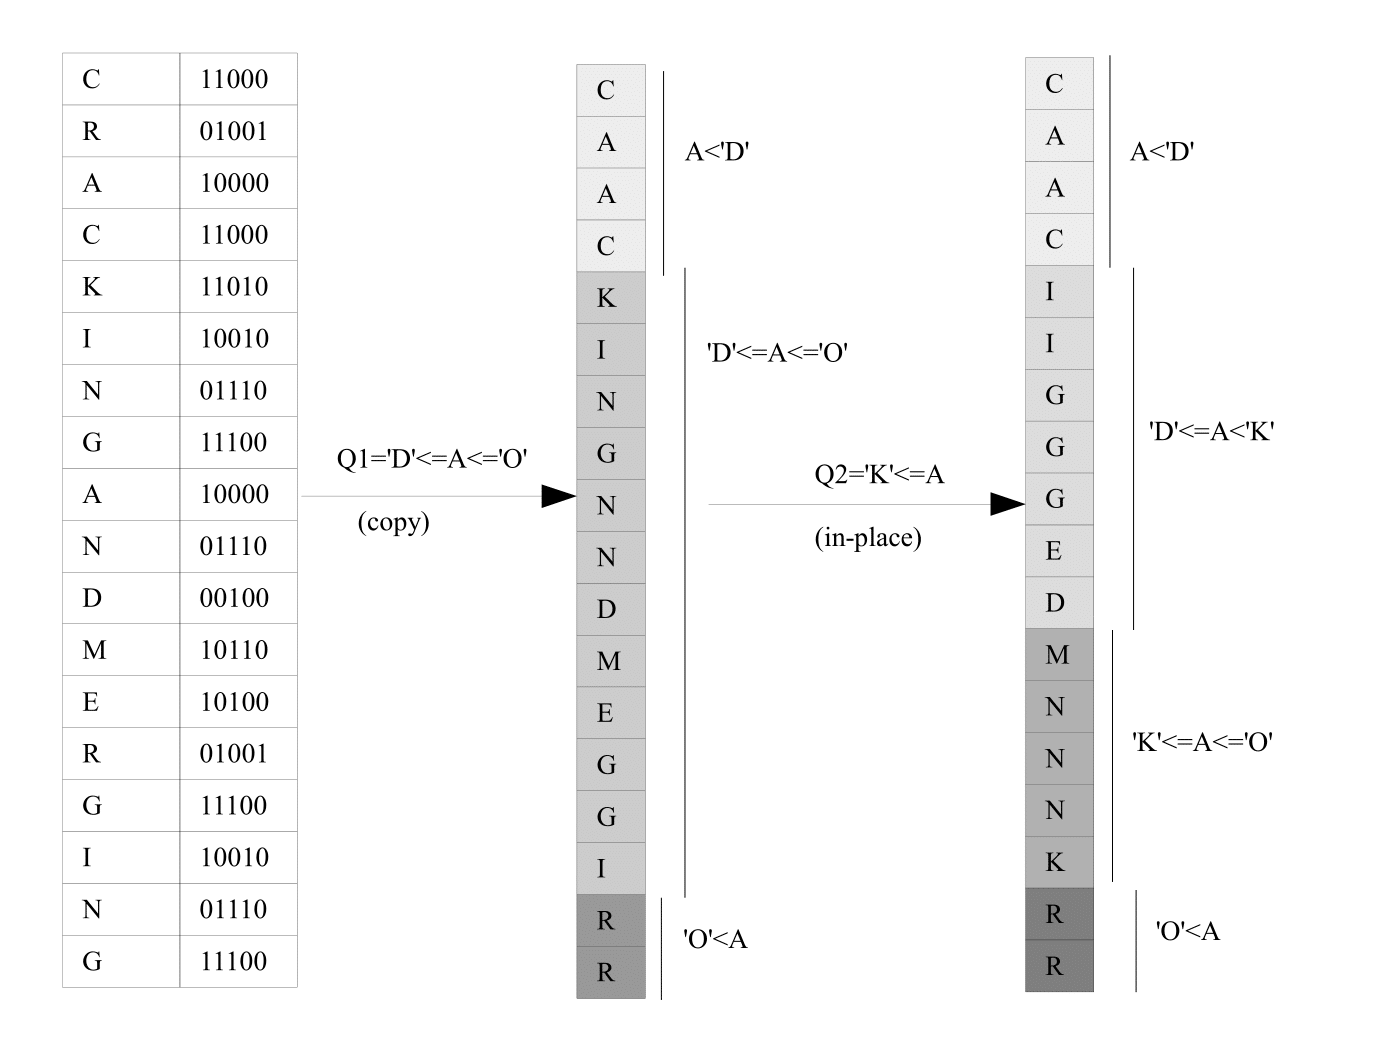
\includegraphics[width=\columnwidth]{cracking.png}
\caption{Cracking a column (adapted from \cite{cracking})}
\end{figure}

\subsection{Analysis and Criticism}
\label{subsec:crack_analysis}
\textbf{Analysis}. In order to analyze database cracking, we compare this approach to a full index and a full scan on a respective column.\\
\begin{itemize}
\item{Costs of Initial Run:} \\High creation costs are the main concern of a full index. While using full index, query processing can start only after initial index creation. Database cracking offers significant imporvements to avoid full sort of an index column. Initial run happens as the first query arrives. In general, first crack takes longer than full scan, as cracking invests some time in indexing. However, cracking still needs less time for initial run than full index to sort the data \cite{survey_cracking}.\\
\item{Costs of Query Processing:} \\After being created, full index processes new queries fast, utilizing advantages of index structures. Full scan takes on average same time to process each next query as it scans the whole table to find relevant tuples. Apart from first query, database cracking performs better than full scan and incrementally reaches the performance of a full index \cite{survey_cracking}.\\
\item{Convergence Towards Full Index:} \\As mentioned in previous point, database cracking constantly narrows its performance towards the full index. It is achieved by incrementally sorting the cracked column when new queries arrive. Consequently, cracked column converges towards full index after number of queries. Clearly, the quality of a cracking step highly depends on the split line defined by query's range. Thus, it is hard to predict how soon query response time of cracking will be reasonably close to one of the full index. On average, after 1,000 queries, query response time of standard cracking is still about 40\% higher than of full index \cite{eval2}.\\
\end{itemize}

\textbf{Criticism}. Several weaknesses of database cracking were outlined in the past. Apart from slow convergence towards full index, they include unpredictable query response time, worse performance with growing number of projected attributes, and not suitable implementation for block-access storage. In \cite{survey_cracking}, Schuhknecht reviewed several approaches such as Vectorized \cite{eval1}, Hybrid \cite{hybrid}, Sideways \cite{sideway} and Stochastic \cite{stochastic} cracking, that try to solve these problems. However, one of the key problems of database cracking: slow convergence, remains unsolved. This concern motivated the development of a further adaptive indexing method: \emph{adaptive merging}, which we present in the next section.

\section{Adaptive Merging}
\label{sec:merging}
In Section~\ref{sec:cracking}, we presented a pioneering approach for adaptive indexing, known as database cracking. We outlined some issues related to this method. In following subsections, we present another adaptive technique for index creation, known as adaptive merging, that tackles unsolved issues of database cracking \cite{merging}. In Subsection~\ref{subsec:merging_idea}, we present motivation and main idea behind adaptive merging. In Subection~\ref{subsec:st_merging}, we describe the approach, followed by an example in Figure 3 and in Subsection~\ref{subsec:merging_analysis}, we conclude the section with some analysis of this method.

\subsection{Motivation and Basic Idea}
\label{subsec:merging_idea}
\textbf{Motivation}. Creators of adaptive merging, Graefe and Harumi, outlined four main weaknesses of database cracking that motivated their research \cite{merging}:
\begin{enumerate}
\item{Slow convergence towards full index.}
\item{Efficiency of cracking depends on query pattern.}
\item{Query response time never reaches that of full index, when cracked column has minimal number of unsorted partitions.}
\item{Database cracking is well-suited for in-memory databases but not for block-access storage.}
\end{enumerate}

\textbf{Main Idea}. Graefe and Harumi proposed adaptive merging, new technique that combines the efficiency of traditional B-tree creation with adaptive nature of database cracking. As its name suggests, adaptive merging is based on merging (as used in merge sort) rather than on partitioning (as used in quicksort and database cracking) \cite{merging}. This new technique promises better query response time and quicker adaption to the new data and new query patterns that database cracking.

\subsection{Adaptive Merging}
\label{subsec:st_merging}
\textbf{Main Idea}: \textit{exploit partitioned B-trees \cite{partitionedtrees} by merging key ranges relevant to actual queries, aiming to reach a desired state and have only a single partition.}\\

\textbf{Steps of Adaptive Merging} 
\begin{enumerate}
\item{Index Selection:}\\
If a column is referred by query for the first time, a new index is created by copying values of a column. \\
\item{Initial Index Creation:}\\
These values are loaded into a number of sorted partitions of predefined size. \\
\item{Index Refinement:}\\
When a column is used for the second time, the query scans one or multiple partitions for a desired key range. It is done by efficiently finding the low end of the range and then scanning to the high end. Several sorted streams of values, resulting in this step, will be merged into a single sorted stream that will be written into a new partition. Moreover, this stream is returned as a result of given query.\\
\item{Overlapping Key Ranges:}\\
Same as in database cracking, ranges of further queries may be fully included in already existing partitions, lay outside of them, or only part of new range is included in existing partitions. Following strategy is applied in these cases:
\begin{itemize}
\item{New query range is a subset of previous query: }
Peform efficient search in a partitioned B-tree.\\
\item{New and old query ranges do not overlap: }
Perform Step 3, create new partition and return it as a result.\\
\item{New and old query ranges partially overlap: }
Split new range into overlapping and non-overlapping sub-ranges. For overlapping subranges perform search in a partitioned B-tree. For non-overlapping subrange perform Step 3 and create new partition for further queries.\\
\end{itemize}
\item{Storage of Reorganization Information:}\\
Like in database cracking, some data structure is required to retain information about performed reorganization. In contrast to a cracker index used in database cracking, the data structure in adaptive merging contains a range of identifiers for the partitions in which given range of keys can be found. As numerous partitions can contain given key range, list of partitions with this key range has to be stored.
\end{enumerate}

\begin{figure}[h]
\centering
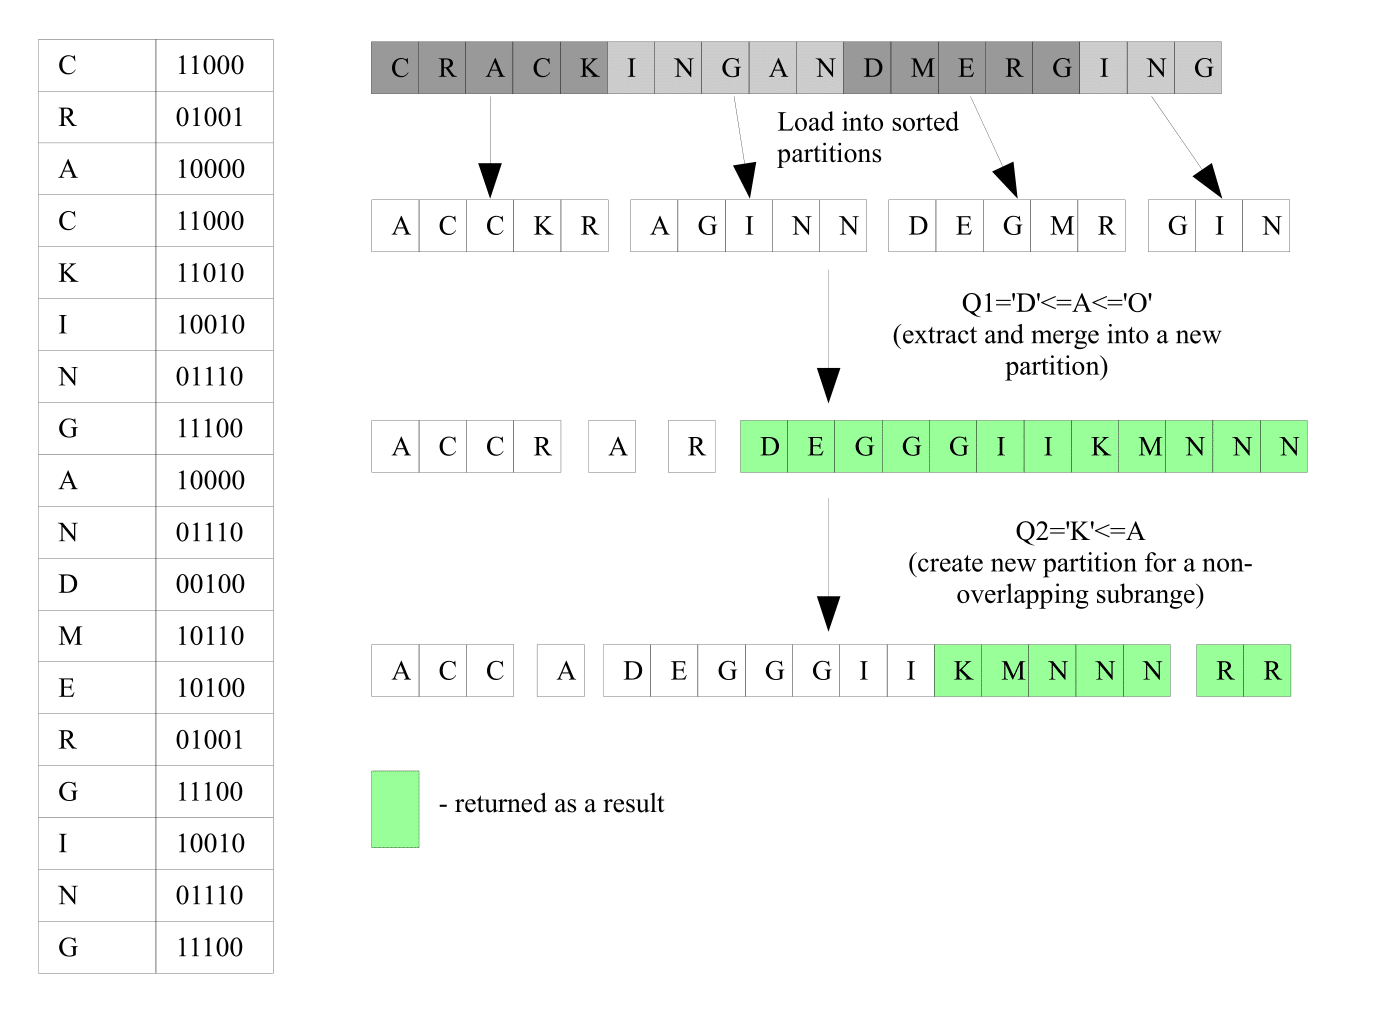
\includegraphics[width=\columnwidth]{merging.png}
\caption{Example for adaptive merging (adapted from \cite{merging})}
\end{figure}

\subsection{Analysis and Criticism}
\label{subsec:merging_analysis}
\textbf{Analysis}. In order to analyze adaptive merging, we compare this approach to database cracking.\\
\begin{itemize}
\item{Cost of Query Processing:} \\Similarly to database cracking, the overhead of the first query is large, as the whole domain has to be scanned and partitioned. However, overhead of query processing by adaptive merging decreases faster than that of database cracking. This can be explained by following:\\
\begin{enumerate}
\item{Fast convergence}: In order to divide 10,000,000 records into partitions with appr. 1,000 entries requires at least 9,999 partitioning keys. As each query provides at most two new split lines, to reach this aim, database cracking requires around 5,000 queries. On the other hand, adaptive merging creates a fully optimized B-tree after 40 queries, reaching the behavior of a full index \cite{merging}.
\item{Sorted partitions}: Sorted partitions in adaptive merging enable lower query response time even if B-tree is not fully optimized. In database cracking, although new range query may completely lie in already existing partition, cracking must be performed. As partition is unsorted, distribution of relevant elements for new query in existing partition is unknown. On the other hand, sorted partitions in adaptive merging enable fast search for the position of a lower key in a partition and scan of entries till higher value.\\
\end{enumerate}
\item{Block-Access Storage:} \\ In contrast to database cracking, designed for in-memory databases, adaptive merging enables adaptive index creation in large data warehouses on external storages. Similarly to traditional B-trees and external merge sort, adaptive merging can be applied to partitioned B-trees and used in block-access storage \cite{merging}. \\
\end{itemize}

\textbf{Issues}. Although adaptive merging matches and may even exceed query response time of full index after a small number of queries, its performance over first queries is concerning. While database cracking matches the scan performance with the second query and exceeds it after the third, adaptive merging needs around 7 queries to exceed the scan time. The first query may be nearly 5 times slower than a scan \cite{hybrid}.

\section{Hybrid Approaches}
\label{sec:hybrid}
In the previous sections, we revisited two fundamental approaches for adaptive indexing: database cracking and adaptive merging. In this section we present further approaches that try to combine strength of both database cracking and adaptive merging. In Subsection~\ref{subsec:hybrid_motiv} we discuss the main idea behind hybrid methods. Later, in Subsection~\ref{subsec:hybrid_strat}, we review main components of an algorithm for adaptive indexing and discuss how these components can be combined to develop a hybrid algorithm for adaptive indexing. To conclude this section, we present existing hybrid approaches followed by examples to provide better understanding of the concept.

\begin{figure}[h]
\centering
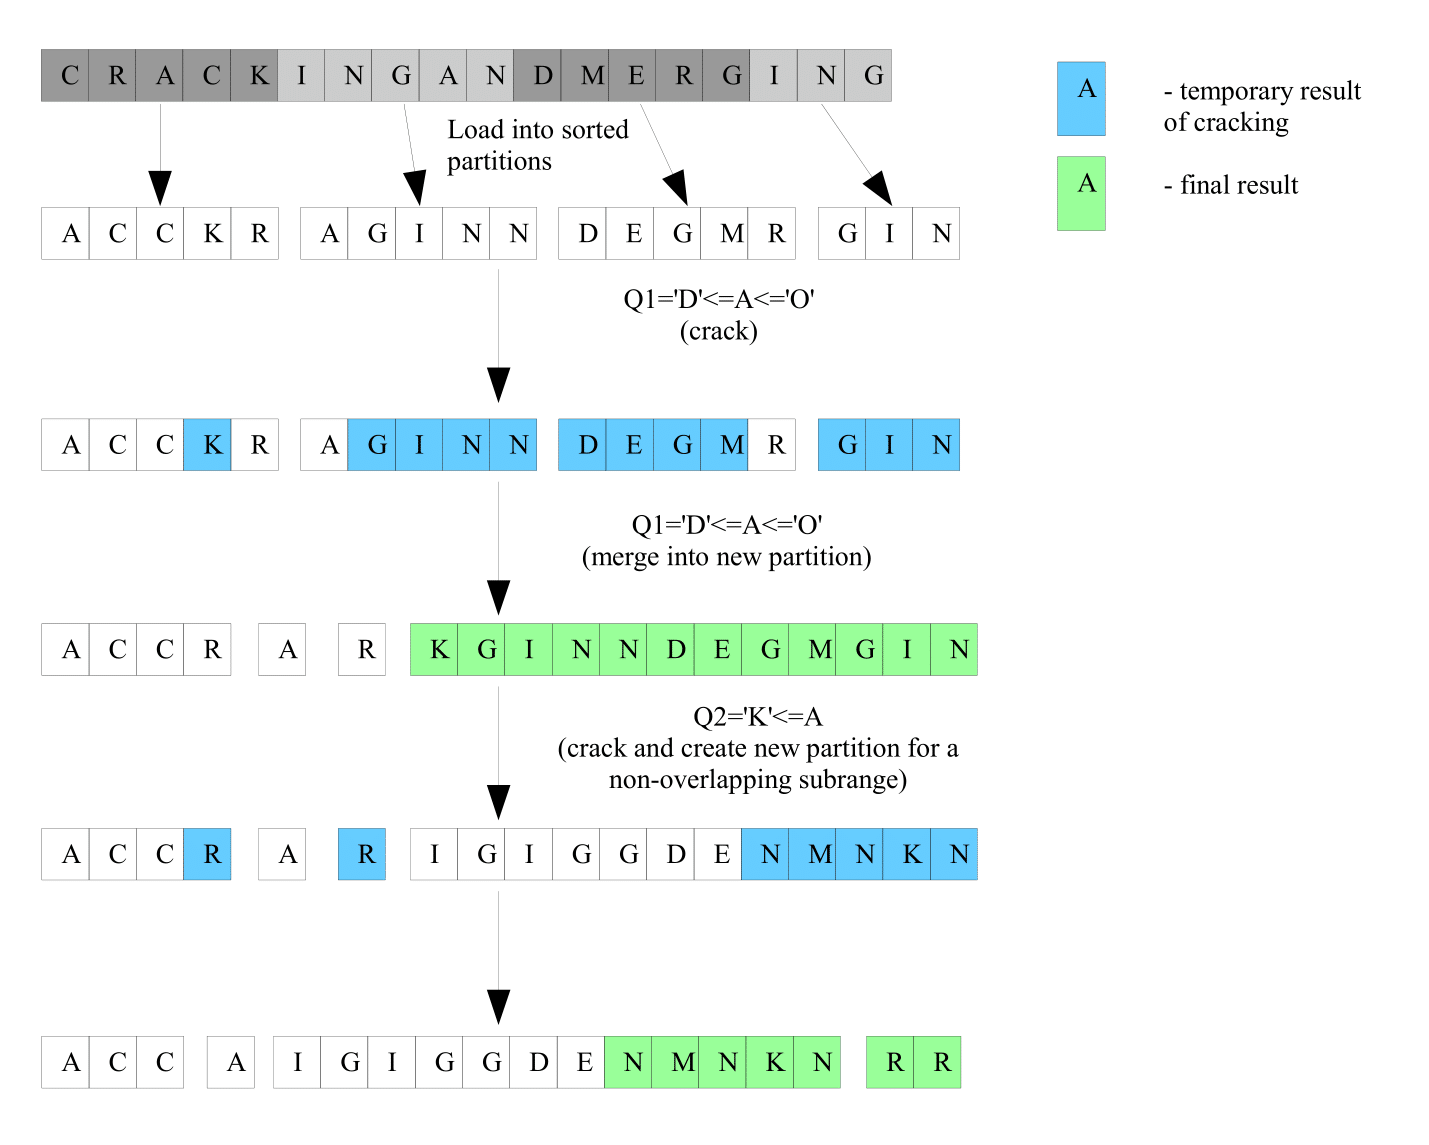
\includegraphics[width=\columnwidth]{hsc.png}
\caption{Hybrid Sort-Sort Algorithm}
\end{figure}

\subsection{Motivation}
\label{subsec:hybrid_motiv}
In previous sections, we revealed two key criteria that adaptive indexing algorithms are judged by: (1) initialization costs for the first query and (2) the number of queries needed to reach the performance of a perfect (full) index. As for (1), it is desired that the initialization does not require more costs than a full scan. And as for (2), one wants to converge towards full index as fast as possible, while performing lightweighted operations during query processing. Based on analysis of database cracking and adaptive merging, we find the strengths of cracking and merging complementary. Database cracking performs lightweighted partitioning to keep initialization costs low, but requires a lot of time to reach the performance of a full index. On the other hand, adaptive merging aims to achieve the behavior of a full index as fast as possible while performing costly operation of sorting both while loading the data into initial and final partitions \cite{hybrid}. In the next subsection, we reveal the sources of their strength and how they can be combined.

\subsection{Strategy}
\label{subsec:hybrid_strat}
The main difference between database cracking and adaptive merging is in the way how initial and final partitions are organized. In \cite{hybrid}, three key methods were presented:
\begin{itemize}
\item{Sorting:} \\
Adaptive merging uses sorting for both the initial and the final partitions. Sorting the initial partition leads to huge costs of initial run that adaptive merging has been criticised for. On the other hand, sorting a final partition is less costly, as it is only performed on a subset of data defined by a query.\\
\item{Cracking: } \\
As used in database cracking, this organization step requires minimal investments, as only two or three partitions are being created. However, because of that and the fact, that new partitions remain unsorted, database cracking is slow in reaching the performance of a full index.\\
\item{Radix-Clustering: } \\
In contrast to sorting, this way of partition organization is more lightweighted which helps to reduce organization costs. Although, radix-clustering doesn't produce fully sorted partitions, it still brings more order to the partitions than cracking.\\
\end{itemize}

\textbf{Hybrid Algorithm Design}. Each of the mentioned organization techniques can be applied both to the initial and final partitions. Consequently, nine potential combinations can be created: starting with Sort-Sort (which is adaptive merging) and ending by Crack-Crack (which is a slight modification of database cracking) \cite{hybrid}.

\subsection{Hybrid Algorithms}
\label{subsec:hybrid_algo}
After presenting the design of hybrid algorithms, we will review nine existing approaches and present some of them in Figures 4, 5, and 6. Furthermore, we will try to narrow the research field to a couple of algorithms that promise improvements on the current adaptive indexing algorithms and discuss their key properties.
\begin{enumerate}
\item{Sort-* Algorithms:} \\
Fully sorting the initial partition is the reason why overhead for initial run is so high by adaptive merging. In fact, sorting takes about 80\% of the time of the first query processing \cite{hybrid}. As a result, none of 3 algorithms (Sort-Sort, Sort-Radix, Sort-Crack) will provide the desired behavior, specifically low initialization costs.\\

\begin{figure}[h]
\centering
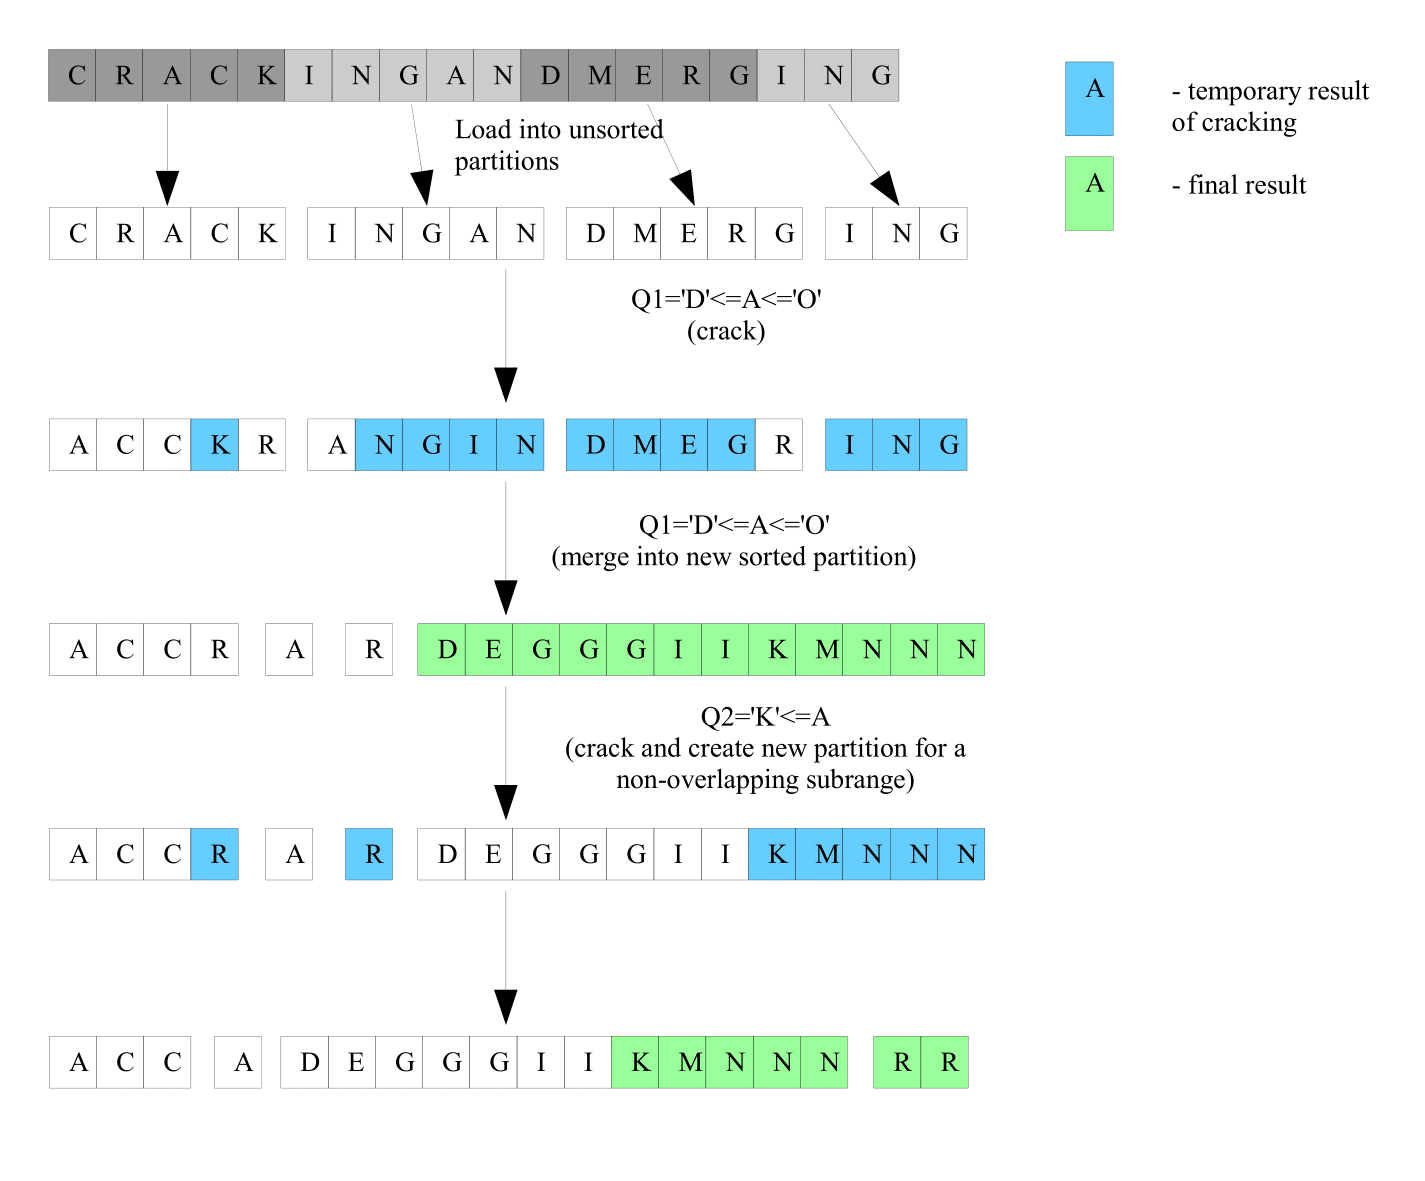
\includegraphics[width=\columnwidth]{hcs.png}
\caption{Hybrid Crack-Sort Algorithm}
\end{figure}

\item{Crack-* Algorithms:}
\begin{itemize}
\item{Crack-Crack:}\\
This modification of database cracking improves over standard cracking in a way that initialization costs are never higher than the ones of the full scan. It is achieved by performing cracking on parts of the column at a time and by creating and cracking initial partitions in one go, instead of copying and then cracking as in plain database cracking. Although, Crack-Crack algorithm significantly improves over standard database cracking, it does not solve the main issue: slow convergence, as it maintains the smooth behavior of cracking.\\
\item{Crack-Sort:}\\
Crack-Sort solves this problem by sorting the final partitions as done in adaptive merging. This allows the algorithm to achieve same costs for the first query as original cracking and fast convergence of adaptive merging. Although this behavior matches the desired one, Crack Sort sacrifices the fast initial run of Crack-Crack and is slower than the scan for the first couple of queries\\
\item{Crack-Radix:}\\
This hybrid approach achieves balanced behavior between the previous hybrids. It achieves similar performance as Crack-Crack at the beginning of the workload and similarly to Crack-Sort it achieves a significant boost in performance. Although it does not achieve the performance of adaptive merging of Crack-Sort, Crack-Radix still significantly improves over plain cracking. Thus, Crack-Radix achieves a nice balance between database cracking and adaptive merging.\\
\end{itemize}
\item{Radix-* Algorithms:}\\
Although costs for first couple of queries for this group of hybrid approaches are slightly higher than the ones of Crack-* approaches, Radix-* approaches significantly improve on adaptive merging in this regard. What is more, organization techniques of final partitions can exploit the extra information provided by clustering to quickly place relevant values. This helps Radix-* approaches to come closer to the convergence behavior of adaptive merging.
\end{enumerate}

\begin{figure}[h]
\centering
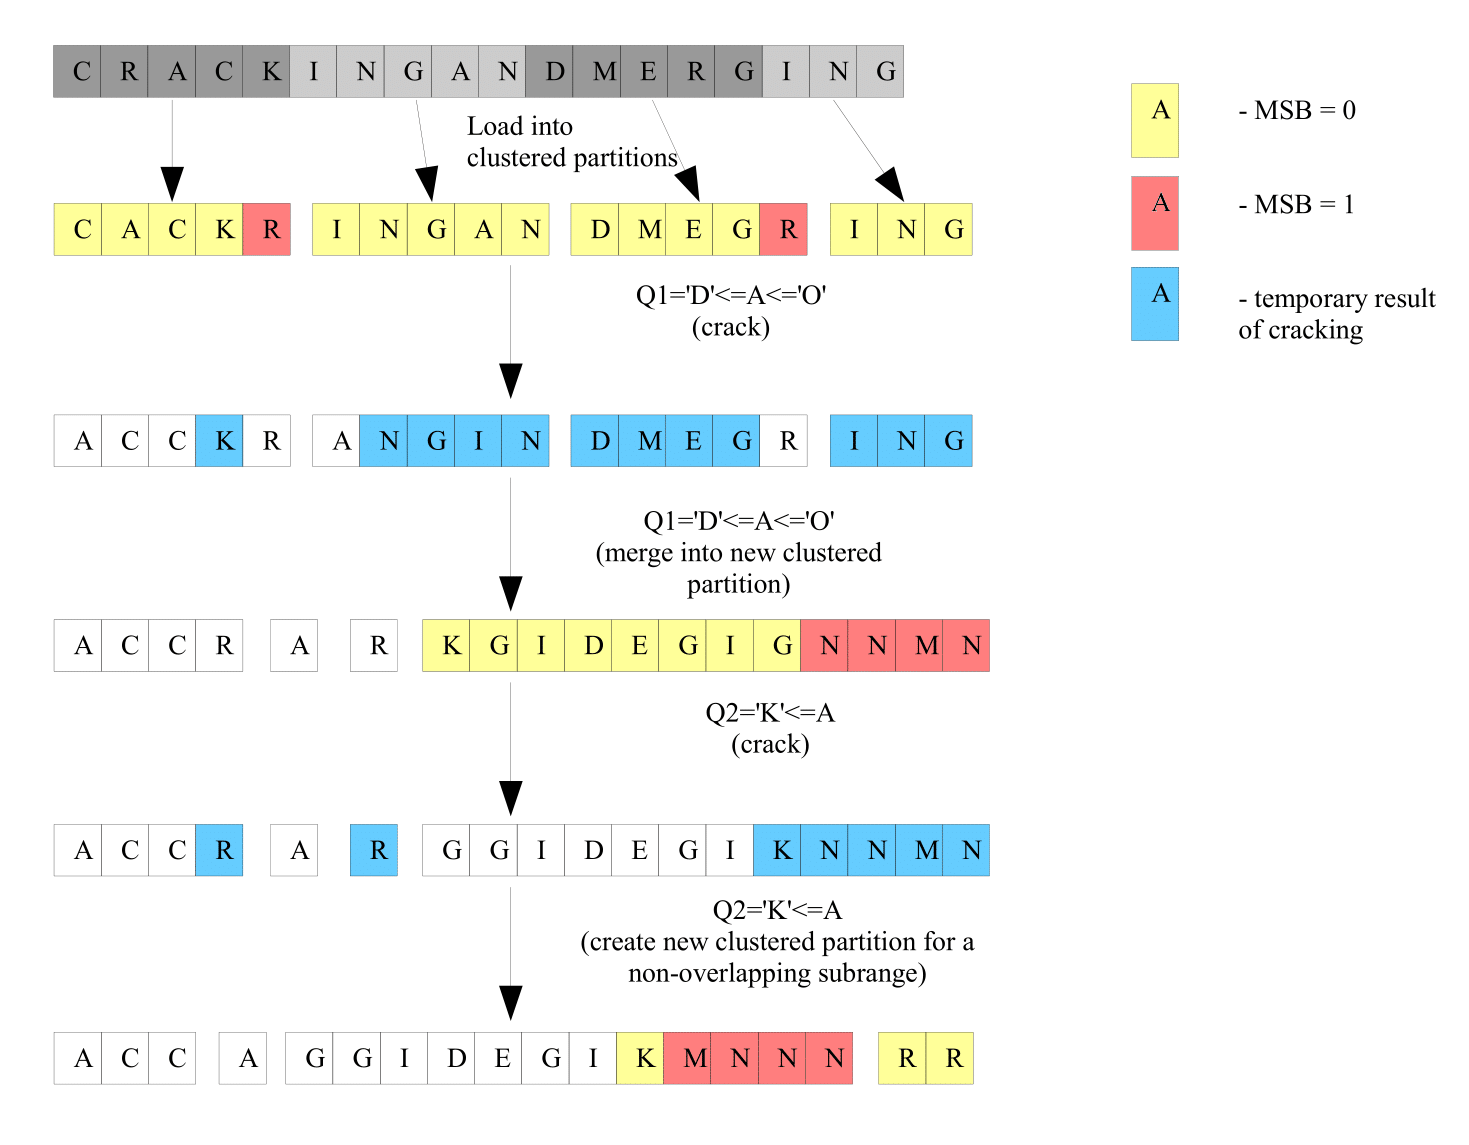
\includegraphics[width=\columnwidth]{hrr.png}
\caption{Hybrid Radix-Radix Algorithm}
\end{figure}

\textbf{Summary.} Crack-* and Radix-* algorithms show promising results. Crack-* methods approach desired behavior by minimizing the costs of initial run by using lightweighted operations of cracking and keeping fast convergence of adaptive merging. Radix-* approaches achieve this goal from other angle: although they use a more expensive operation of clustering to create initial partitions, the information about created clusters help to minimize the costs for organizing final partitions.

\section{Lessons Learned \& Future Work}
\label{sec:eval}
In this section we will put together the major lessons learned in this paper and outline further interesting research possibilities.
\begin{itemize}
\item{\textbf{Lessons Learned}}
\begin{enumerate}
\item{Adaptive Indexing Is a Promising Concept:}\\
Numerous researches has shown that adaptive indexing is a valid alternative to the state-of-art in database indexing. Adaptive approaches tackle numerous indexing issues like growing workload, unpredictable behavior of the user, while using rather simple concepts. Various independent studies have shown that database cracking is repeatable and can be integrated in existing DBMSs, while making straight-forward changes \cite{cracking}.\\
\item{Database Cracking and Adaptive Merging Have Similar Nature:}\\
Adaptive merging seemed to use a differing approach to reach same goal as database cracking. In contrast to partitioning, used in cracking, it uses merging to create final partitions. Furthermore, adaptive merging uses another underlying datastructure to store reorganization progress (partitioned B-Tree in contrast to AVL-Tree). However, as shown in \cite{hybrid}, adaptive merging and database cracking have much in common and their complementary nature can be used to develop further approaches for adaptive indexing.\\
\item{Crack-Sort and Crack-Radix Are Valid Alternatives:}\\
As discussed before, different combinations of reorganization techniques for initial and final partitions produce hybrid approaches, some of which are valid alternatives to database cracking and adaptive merging. While Sort-* approaches have proved to be rather inefficient and do not reach desired behavior, Crack-* approaches provide a nice balance between cracking and adaptive merging and utilize strength of both approaches. Especially, Crack-Sort and Crack-Radix, both of which have the lighweighted initialization of database cracking and rapid convergence of adaptive merging. Both approaches can be used depending on the task: Crack-Radix can be used to provide a more smooth convergence, while Crack-Sort can be used when fast adaptation is needed.\\
\item{Hybrid Algorithms Can Be Combined:}\\
Presented hybrid algorithms can be optimized, e.g. by finding optimal clustering degree for Radix-* approaches, applying multi-level merging from adaptive merging. Another promising optimization possibility is to provide a functionality to combine various hybrid approaches \cite{hybrid}. For example, Crack-Radix can be used for first part of the workload as it provides a rather smooth adaption behavior, never being slower than a full scan. Later, Crack-Sort can be used to force eager index optimization.\\
\end{enumerate}
\item{\textbf{Future Work}}
\begin{enumerate}
\item{Further Research on Adaptive Merging and Hybrid Approaches Needed:}\\
Database cracking has been thoroughly studied and numerous issues of this approach have been found: slow convergence towards full index, unpredictable query response time, worse performance with growing number of projected attributes, and not suitable implementation for block-access storage. These open questions motivated further research and development of modificated approaches such as vectorized, sideways, stochastic cracking, and hybrid approaches. We think that adaptive merging and other hybrid approaches can benefit from further research. Several aspects remain unclear: do hybrid approaches provide robust tuple reconstruction; how sensitive are they to different query patterns; how can these methods be combined with modern indexing trends like \emph{sorting radix sort} or \emph{Adaptive Radix Trees} \cite{art}? \\
\item{New Strategies for Hybrid Algorithms:}\\
Previously presented hybrid approaches were constructed by following same strategy: load data into initial and final partitions following one of three organization techniques: Sorting, Cracking, and Radix-Clustering. However, this approach restricts the number of possible hybrids. It is possible, that hybrid approaches constructed using other techniques can produce better results.\\
\item{Influence of Underlying Datastructures:}\\
In previous sections, we discussed that database cracking and adaptive merging use different underlying structures to store reorganization progress: the former uses AVL-Tree, the latter uses partitioned B-Trees. The influences of these datastructures on the performance of respective algorithms has not been studied yet. The introduction of new indexing datastructures, such as Adaptive Radix Trees or Self Pruning Splay Trees \cite{spst}, promise siginificant improvement in performance for database cracking. Both of these datastructures enable faster lookup. However, their compatibility with adaptive merging and hybrid approaches remain unclear.\\
\item{Integration of Adaptive Indexing in Other Models:}\\
Adaptive indexing has nice background to be used in column-oriented databases. However, the aspects of adaptive indexing in other database architectures remain unclear. Some modifications have been proposed to make database cracking usable in row-oriented databases \cite{cracking}. However, this direction has not been further researched. Same applies to other database architectures, such as graph databases. Modifications required to use other methods for adaptive indexing, like hybrid methods of adaptive merging, have to be researched.
\end{enumerate}
\end{itemize}

%\section{Related Work}
%\label{sec:rel}
%Some research on related work has to be done.

\section{Conclusions}
\label{sec:conc}
In this paper we introduced the concept of adaptive indexing. We discussed \emph{partial} and \emph{soft} indexes that provide background for adaptive indexing. We revisited two fundamental approaches for adaptive indexing: \emph{database cracking} and \emph{adaptive merging}. Furthermore, we showed, how strength of these methods can be combined to develop \emph{hybrid approaches} that try to reach the performance of a perfect hybrid: lightweighted initialization and fast convergence towards full index.

We hope that this paper will give necessary background information on adaptive indexing and motivates further research in this field of database technologies.

\section*{Acknowledgement}
I thank Gabriel Campero Durand of Otto-von-Guericke-University, Magdeburg for providing insight and expertise to start this research and for his enormous support throughout the whole process of research, writing and evaluation of this scientific work. I would also like to show my gratitude to the DBSE Research Group of Otto-von-Guericke-University, Magdeburg for making this work possible and organising the ``Seminar on Modern Software Engineering and Database Concepts'', during which this research took place.

\begin{thebibliography}{8}

\bibitem{partial1}
Stonebraker, Michael. "The case for partial indexes." Sigmod Record 18.4, 1989.
\bibitem{partial2}
Seshadri, Praveen, and Arun Swami. "Generalized partial indexes." Data Engineering, 1995. Proceedings of the Eleventh International Conference on. IEEE, 1995.
\bibitem{soft_indexes}
L\"uhring, Martin, et al. "Autonomous management of soft indexes." Data Engineering Workshop, 2007 IEEE 23rd International Conference on. IEEE, 2007.
\bibitem{cracking}
Idreos, Stratos, Martin L. Kersten, and Stefan Manegold. "Database Cracking." CIDR. Vol. 7. 2007.
\bibitem{survey_cracking}
Schuhknecht, Felix Martin. "Closing the circle of algorithmic and system-centric database optimization: a comprehensive survey on adaptive indexing, data partitioning, and the rewiring of virtual memory.", 2016.
\bibitem{merging}
Graefe, Goetz, and Harumi Kuno. "Self-selecting, self-tuning, incrementally optimized indexes." Proceedings of the 13th International Conference on Extending Database Technology. ACM, 2010.
\bibitem{partitionedtrees}
Graefe, Goetz. "Sorting and indexing with partitioned B-trees". CIDR, 2003.
\bibitem{hybrid}
Idreos, Stratos, et al. "Merging what's cracked, cracking what's merged: adaptive indexing in main-memory column-stores." Proceedings of the VLDB Endowment 4.9, 2011.
\bibitem{eval1}
Pirk, Holger, et al. "Database cracking: fancy scan, not poor man's sort!." Proceedings of the Tenth International Workshop on Data Management on New Hardware. ACM, 2014.
\bibitem{eval2}
Schuhknecht, Felix Martin, Alekh Jindal, and Jens Dittrich. "The uncracked pieces in database cracking." Proceedings of the VLDB Endowment 7.2 (2013): 97-108.
\bibitem{defin}
Idreos, Stratos, Stefan Manegold, and Goetz Graefe. "Adaptive indexing in modern database kernels." Proceedings of the 15th International Conference on Extending Database Technology. ACM, 2012.
\bibitem{sideway}
Idreos, Stratos, Martin L. Kersten, and Stefan Manegold. "Self-organizing tuple reconstruction in column-stores." Proceedings of the 2009 ACM SIGMOD International Conference on Management of data. ACM, 2009.
\bibitem{stochastic}
Halim, Felix, et al. "Stochastic database cracking: Towards robust adaptive indexing in main-memory column-stores." Proceedings of the VLDB Endowment 5.6 (2012): 502-513.
\bibitem{art}
V. Leis et al. "The Adaptive Radix Tree: ARTful Indexing for
Main-Memory Databases." In ICDE, 2013.
\bibitem{spst}
Holanda, Pedro Thiago Timbó. "SPST-Index: a self pruning splay tree index for database cracking.", 2017.

\end{thebibliography}

\end{document}
